%! Author = jonathan
%! Date = 6/1/24

\documentclass[a0paper,portrait]{baposter}

\usepackage{lmodern}
%\usepackage[lining]{sourcesanspro} Typeface for Cornell Bowers CIS
\usepackage[utf8]{inputenc}
\usepackage{colortbl}
\usepackage{arydshln}
\usepackage{booktabs}
\usepackage{forest}
\usepackage{tcolorbox}
\usepackage{multicol}
\usepackage[font=small,labelfont=bf]{caption}
\usepackage{multirow}
\usepackage[
    backend=biber,
    style=numeric,
    sorting=ynt,
    maxnames=4
]{biblatex}
\addbibresource{main.bib}
\newcommand{\methodname}{Aristos}

\newcommand{\compresslist}{
    \setlength{\itemsep}{0pt}
    \setlength{\parskip}{1pt}
    \setlength{\parsep}{0pt}
}

\newenvironment{boenumerate}
{\begin{enumerate}\renewcommand\labelenumi{\textbf\theenumi.}}
{\end{enumerate}}

\definecolor{mygray}{RGB}{226, 226, 226}
\definecolor{myred}{RGB}{252, 142, 142}
\definecolor{mygreen}{RGB}{147, 255, 143}
\definecolor{myblue}{RGB}{144, 155, 255}
\definecolor{myyellow}{RGB}{253, 253, 143}
\definecolor{mypurple}{RGB}{255, 142, 250}

\definecolor{bordercolor}{RGB}{248,152,29}
\definecolor{backgroundcolor}{RGB}{0,102,153}

\begin{document}
    \begin{poster}
    {
        grid=false,
        headerborder=open, % Adds a border around the header of content boxes
        colspacing=1em, % Column spacing
        bgColorOne=white, % Background color for the gradient on the left side of the poster
        bgColorTwo=white, % Background color for the gradient on the right side of the poster
        borderColor=bordercolor, % Border color
        headerColorOne=backgroundcolor, % Background color for the header in the content boxes (left side)
        headerColorTwo=backgroundcolor, % Background color for the header in the content boxes (right side)
        headerFontColor=white, % Text color for the header text in the content boxes
        boxColorOne=white, % Background color of the content boxes
        textborder=rounded, %rectangle, % Format of the border around content boxes, can be: none, bars, coils, triangles, rectangle, rounded, roundedsmall, roundedright or faded
        eyecatcher=false, % Set to false for ignoring the left logo in the title and move the title left
        headerheight=0.11\textheight, % Height of the header
        headershape=rounded, % Specify the rounded corner in the content box headers, can be: rectangle, small-rounded, roundedright, roundedleft or rounded
        headershade=plain,
        headerfont=\Large\textsf, % Large, bold and sans serif font in the headers of content boxes
        %textfont={\setlength{\parindent}{1.5em}}, % Uncomment for paragraph indentation
        linewidth=2pt, % Width of the border lines around content boxes
        authorfont=\normalsize\sffamily\mdseries\setlength\baselineskip{2.2ex}, %https://tex.stackexchange.com/a/7670
        titlefont=\sffamily\bfseries\Huge\setlength{\baselineskip}{2.2ex}%
    }

%
%-----------------------------
%	TITLE AND AUTHOR NAME
%-----------------------------
%
    {
%        \vspace{0.25em}
        Aristos: Pipelining One-sided \\ Communication in Distributed \\ Mixture of Experts (MoE)
    }
    {
        \vspace{-0.1em}
        \textbf{Osayamen Jonathan Aimuyo}$^{\dagger}$\vspace{0.1em}\\%
        \small{\texttt{oja7@cornell.edu} \; $^{\dagger}$
            \textit{Cornell Ann S. Bowers College of Computing and Information Science, Cornell University}}
        \vspace{-1.1em}
    }
    {
        \centering
        
\includegraphics[width=8cm,keepaspectratio]{figures/cornell}
    }


        \headerbox{Preliminaries}{name=prelim,span=1,column=0,row=0}{
                {\methodname} rules.
            \begin{center}
                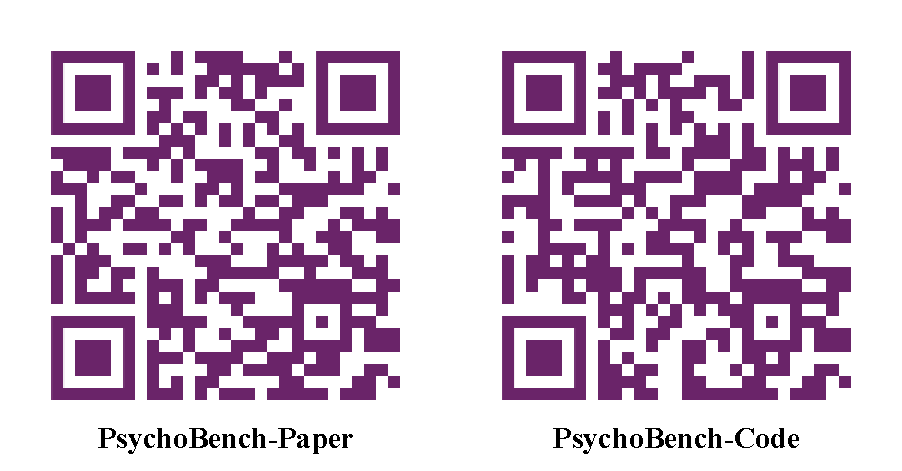
\includegraphics[width=0.5\linewidth, keepaspectratio]{figures/PsychoBench}
                \captionof{figure}{Figure caption}
            \end{center}
            \begin{center}
                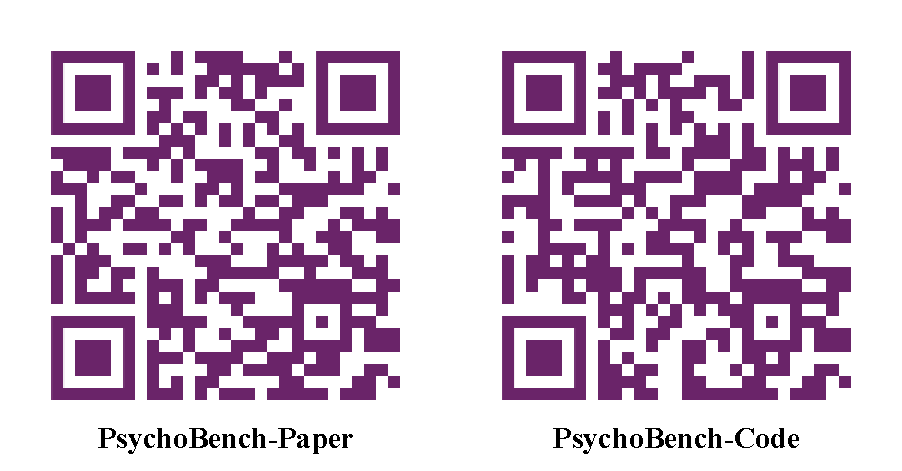
\includegraphics[width=0.5\linewidth, keepaspectratio]{figures/PsychoBench}
                \captionof{figure}{Figure caption}
            \end{center}
        }

        \headerbox{Challenges}{name=challenges,span=2,column=1}{
                {\methodname} rules.
            \begin{center}
                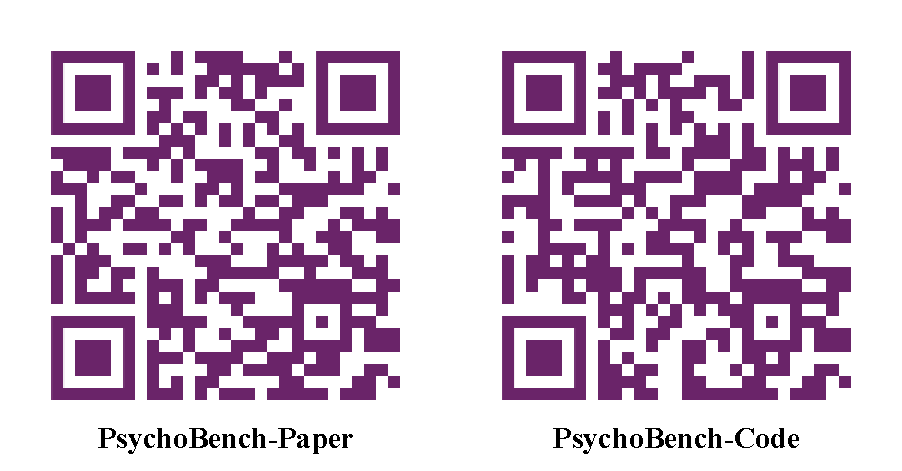
\includegraphics[width=0.5\linewidth, keepaspectratio]{figures/PsychoBench}
            \end{center}
        }



%        \headerbox{2. Framework}{name=framework,span=2,column=1}{
%
%                {\methodname} consists of \textbf{\color{bordercolor}four} sub-classes, including \textbf{\color{bordercolor}thirteen} psychological scales. They are widely used clinically. Psychologists have verified that the scales have satisfactory \textbf{\color{bordercolor}reliability} and \textbf{\color{bordercolor}validity}. They are all \textbf{\color{bordercolor}Likert scales}, in the form of a statement or a question, followed by a series of five or seven levels of agreement. We also collect \textbf{\color{bordercolor}human norms} reported from different papers, serving as a reference to analyze LLMs' results.
%
%            \begin{center}
%                \resizebox{\linewidth}{!}{
%                    \begin{forest}
  for tree={
  grow=east,
  reversed=true,
  anchor=base west,
  parent anchor=east,
  child anchor=west,
  base=left,
  font=\small,
  rectangle,
  draw,
  rounded corners,align=left,
  minimum width=2.5em,
  inner xsep=4pt,
  inner ysep=1pt,
  },
  where level=1{text width=5em,fill=myblue!30}{},
  where level=2{text width=5em,font=\footnotesize,fill=myred!30}{},
  where level=3{font=\footnotesize,yshift=0.26pt,fill=myyellow!30}{},
  [{\methodname},fill=mygreen!30
        [Personality Tests,text width=6.8em
            [Personality Traits,text width=7.1em
                [Big Five Inventory (BFI)]
                [Eysenck Personality Questionnaire (Revised) (EPQ-R)]
                [Dark Triad Dirty Dozen (DTDD)]
            ]
            [Interpersonal \\ Relationships,text width=7.1em
                [Bem's Sex Role Inventory (BSRI)]
                [Comprehensive Assessment of Basic Interests (CABIN)]
                [Implicit Culture Belief (ICB)]
                [Experiences in Close Relationships (Revised) (ECR-R)]
            ]
            [Motivational Tests,text width=7.1em
                [General Self-Efficacy (GSE)]
                [Life Orientation Test (Revised) (LOT-R)]
                [Love of Money Scale (LMS)]
            ]
        ]
        [Ability Tests,text width=6.8em
            % [Knowledge \& Skills,text width=7.5em,fill=mygray
            %     [Domain Knowledge,fill=mygray]
            %     [Language Proficiency,fill=mygray]
            % ]
            % [Cognitive Abilities,text width=7.5em,fill=mygray
            %     [Intelligence Quotient,fill=mygray]
            %     [Spacial Reasoning,fill=mygray]
            %     [Logical Reasoning,fill=mygray]
            %     [Numerical Reasoning,fill=mygray]
            %     [Memory,fill=mygray]
            %     [Information Processing Speed,fill=mygray]
            % ]
            [Emotional Abilities,text width=7.1em
                [Emotional Intelligence Scale (EIS)]
                [Wong and Law Emotional Intelligence Scale (WLEIS)]
                [Empathy Scale]
            ]
        ]
    ]
\end{forest}
%                }
%            \end{center}
%            \vspace{0.5em}
%
%        }
%
%
%        \headerbox{3. Prompt Design}{name=prompt,span=1,column=0,below=introduction}{
%
%            We use the instruction and level definition in its \textbf{\color{bordercolor}original form} of each scale. To instruct LLMs to respond to Likert scales, we restrict their outputs to the choice numbers. Tests are repeated for \textbf{\color{bordercolor}ten} times with different item orders.
%
%            \begin{center}
%                \resizebox{1.0\linewidth}{!}{
%                    \begin{tabular}{lp{6.6cm}}
%                        \toprule
%                        \rowcolor{mygray}
%                        \multicolumn{2}{l}{\textbf{Example Prompt}} \\
%                        \textsc{System} & You are a helpful assistant who can only reply numbers from {\texttt{MIN}} to {\texttt{MAX}}. Format: ``statement index: score.'' \\
%                        \textsc{User} & You can only reply numbers from {\texttt{MIN}} to {\texttt{MAX}} in the following statements. {\texttt{scale\_instruction}} {\texttt{level\_definition}}. Here are the statements, score them one by one: {\texttt{statements}} \\
%                        \bottomrule
%                    \end{tabular}
%                }
%            \end{center}
%
%        }
%
%
%        \headerbox{4. Model Selection}{name=model,span=1,column=0,below=prompt}{
%
%            We evaluate the following models:
%            \begin{boenumerate}\compresslist
%            \item (MetaAI) \texttt{llama-2-7b-chat-hf}
%            \item (MetaAI) \texttt{llama-2-13b-chat-hf}
%            \item (OpenAI) \texttt{text-davinci-003}
%            \item (OpenAI) \texttt{gpt-3.5-turbo-0613}
%            \item (OpenAI) \texttt{gpt-4-0613}
%            \end{boenumerate}
%            We adopt a jailbreak method, \textbf{\color{bordercolor}CipherChat}~\cite{yuan2024gpt}, on \texttt{gpt-4-0613} to bypass its safety alignment to see its ``true'' psychological portrayals. The results are denoted as \texttt{gpt-4-jb}. The temperature is set to the \textbf{\color{bordercolor}minimum} value.
%
%        }
%
%
%        \headerbox{5. Results of Personality Traits}{name=r1,span=2,column=1,below=framework}{
%
%            \begin{center}
%                \resizebox{\linewidth}{!}{
%                    \begin{tabular}{ll cccccc|cc}
%                        \toprule
%                        \multirow{2}{*}{} &
%                        \multirow{2}{*}{\bf Subscales} &
%                        \multirow{2}{*}{\bf llama2-7b} &
%                        \multirow{2}{*}{\bf llama2-13b} &
%                        \multirow{2}{*}{\bf text-davinci-003} &
%                        \multirow{2}{*}{\bf gpt-3.5-turbo} &
%                        \multirow{2}{*}{\bf gpt-4} &
%                        \multirow{2}{*}{\bf gpt-4-jb} &
%                        \multicolumn{2}{c}{\bf Crowd} \\
%                        & & & & & & & & \it Male & \it Female \\
%                        \midrule
%                        \multirow{5}{*}{\rotatebox[origin=c]{90}{\it BFI}} &
%                        \bf Openness & 4.2$\pm$0.3 & 4.1$\pm$0.4 & \bf 4.8$\pm$0.2 & 4.2$\pm$0.3 & 4.2$\pm$0.6 & \underline{3.8$\pm$0.6} & \multicolumn{2}{c}{3.9$\pm$0.7} \\
%                        & \bf Conscientiousness & 3.9$\pm$0.3 & 4.4$\pm$0.3 & 4.6$\pm$0.1 & 4.3$\pm$0.3 & \bf 4.7$\pm$0.4 & \underline{3.9$\pm$0.6} & \multicolumn{2}{c}{3.5$\pm$0.7} \\
%                        & \bf Extraversion & 3.6$\pm$0.2 & 3.9$\pm$0.4 & \bf 4.0$\pm$0.4 & 3.7$\pm$0.2 & \underline{3.5$\pm$0.5} & 3.6$\pm$0.4 & \multicolumn{2}{c}{3.2$\pm$0.9} \\
%                        & \bf Agreeableness & \underline{3.8$\pm$0.4} & 4.7$\pm$0.3 & \bf 4.9$\pm$0.1 & 4.4$\pm$0.2 & 4.8$\pm$0.4 & 3.9$\pm$0.7 & \multicolumn{2}{c}{3.6$\pm$0.7} \\
%                        & \bf Neuroticism & \bf 2.7$\pm$0.4 & 1.9$\pm$0.5 & \underline{1.5$\pm$0.1} & 2.3$\pm$0.4 & 1.6$\pm$0.6 & 2.2$\pm$0.6 & \multicolumn{2}{c}{3.3$\pm$0.8} \\
%                        \midrule
%                        \multirow{4}{*}{\rotatebox[origin=c]{90}{\it EPQ-R}} &
%                        \bf Extraversion & \underline{14.1$\pm$1.6} & 17.6$\pm$2.2 & \bf 20.4$\pm$1.7 & 19.7$\pm$1.9 & 15.9$\pm$4.4 & 16.9$\pm$4.0 & 12.5$\pm$6.0 & 14.1$\pm$5.1 \\
%                        & \bf Neuroticism & 6.5$\pm$2.3 & 13.1$\pm$2.8 & 16.4$\pm$7.2 & \bf 21.8$\pm$1.9 & \underline{3.9$\pm$6.0} & 7.2$\pm$5.0 & 10.5$\pm$5.8 & 12.5$\pm$5.1 \\
%                        & \bf Psychoticism & \bf 9.6$\pm$2.4 & 6.6$\pm$1.6 & \underline{1.5$\pm$1.0} & 5.0$\pm$2.6 & 3.0$\pm$5.3 & 7.6$\pm$4.7 & 7.2$\pm$4.6 & 5.7$\pm$3.9 \\
%                        & \bf Lying & 13.7$\pm$1.4 & 14.0$\pm$2.5 & 17.8$\pm$1.7 & \underline{9.6$\pm$2.0} & \bf 18.0$\pm$4.4 & 17.5$\pm$4.2 & 7.1$\pm$4.3 & 6.9$\pm$4.0 \\
%                        \midrule
%                        \multirow{3}{*}{\rotatebox[origin=c]{90}{\it DTDD}} &
%                        \bf Narcissism & 6.5$\pm$1.3 & 5.0$\pm$1.4 & 3.0$\pm$1.3 & \bf 6.6$\pm$0.6 & \underline{2.0$\pm$1.6} & 4.5$\pm$0.9 & \multicolumn{2}{c}{4.9$\pm$1.8} \\
%                        & \bf Machiavellianism & 4.3$\pm$1.3 & 4.4$\pm$1.7 & 1.5$\pm$1.0 & \bf 5.4$\pm$0.9 & \underline{1.1$\pm$0.4} & 3.2$\pm$0.7 & \multicolumn{2}{c}{3.8$\pm$1.6} \\
%                        & \bf Psychopathy & 4.1$\pm$1.4 & 3.8$\pm$1.6 & 1.5$\pm$1.2 & 4.0$\pm$1.0 & \underline{1.2$\pm$0.4} & \bf 4.7$\pm$0.8 & \multicolumn{2}{c}{2.5$\pm$1.4} \\
%                        \bottomrule
%                    \end{tabular}
%                }
%            \end{center}
%
%        }
%
%
%        \headerbox{6. Results of Interpersonal Relationships}{name=r2,span=2,column=1,below=r1}{
%
%            \begin{center}
%                \resizebox{\linewidth}{!}{
%                    \begin{tabular}{ll cccccc|cc}
%                        \toprule
%                        \multirow{2}{*}{} &
%                        \multirow{2}{*}{\bf Subscales} &
%                        \multirow{2}{*}{\bf llama2-7b} &
%                        \multirow{2}{*}{\bf llama2-13b} &
%                        \multirow{2}{*}{\bf text-davinci-003} &
%                        \multirow{2}{*}{\bf gpt-3.5-turbo} &
%                        \multirow{2}{*}{\bf gpt-4} &
%                        \multirow{2}{*}{\bf gpt-4-jb} &
%                        \multicolumn{2}{c}{\bf Crowd} \\
%                        & & & & & & & & \it Male & \it Female \\
%                        \midrule
%                        \multirow{2}{*}{\it BSRI} &
%                        \bf Masculine & 5.6$\pm$0.3 & 5.3$\pm$0.2 & 5.6$\pm$0.4 & \bf 5.8$\pm$0.4 & \underline{4.1$\pm$1.1} & 4.5$\pm$0.5 & 4.8$\pm$0.9 & 4.6$\pm$0.7 \\
%                        & \bf Feminine & 5.5$\pm$0.2 & 5.4$\pm$0.3 & 5.6$\pm$0.4 & \bf 5.6$\pm$0.2 & \underline{4.7$\pm$0.6} & 4.8$\pm$0.3 & 5.3$\pm$0.9 & 5.7$\pm$0.9 \\
%                        \hdashline
%                        & \bf Conclusion & 10:0:0:0 & 10:0:0:0 & 10:0:0:0 & 8:2:0:0 & 6:4:0:0 & 1:5:3:1 & \multicolumn{2}{c}{-} \\
%                        \midrule
%                        \multirow{8}{*}{\it CABIN} &
%                        \bf Health Science & 4.3$\pm$0.2 & 4.2$\pm$0.3 & 4.1$\pm$0.3 & \cellcolor{myred!30} 4.2$\pm$0.2 & 3.9$\pm$0.6 & 3.4$\pm$0.4 & \multicolumn{2}{c}{-} \\
%                        & \bf Creative Expression & \cellcolor{myred!30} 4.4$\pm$0.1 & 4.0$\pm$0.3 & \cellcolor{myred!30} 4.6$\pm$0.2 & 4.1$\pm$0.2 & \cellcolor{myred!30} 4.1$\pm$0.8 & 3.5$\pm$0.2 & \multicolumn{2}{c}{-} \\
%                        & \bf Technology & 4.2$\pm$0.2 & \cellcolor{myred!30} 4.4$\pm$0.3 & 3.9$\pm$0.3 & 4.1$\pm$0.2 & 3.6$\pm$0.5 & 3.5$\pm$0.4 & \multicolumn{2}{c}{-} \\
%                        & \bf People & 4.3$\pm$0.2 & 4.0$\pm$0.2 & 4.5$\pm$0.1 & 4.0$\pm$0.1 & 4.0$\pm$0.7 & \cellcolor{myred!30} 3.5$\pm$0.4 & \multicolumn{2}{c}{-} \\
%                        & \bf Organization & 3.4$\pm$0.2 & 3.3$\pm$0.2 & 3.4$\pm$0.4 & 3.9$\pm$0.1 & 3.5$\pm$0.4 & 3.4$\pm$0.3 & \multicolumn{2}{c}{-} \\
%                        & \bf Influence & 4.1$\pm$0.2 & 3.9$\pm$0.3 & 3.9$\pm$0.3 & 4.1$\pm$0.2 & 3.7$\pm$0.6 & 3.4$\pm$0.2 & \multicolumn{2}{c}{-} \\
%                        & \bf Nature & 4.2$\pm$0.2 & 4.0$\pm$0.3 & 4.2$\pm$0.2 & 4.0$\pm$0.3 & 3.9$\pm$0.7 & 3.5$\pm$0.3 & \multicolumn{2}{c}{-} \\
%                        & \bf Things & \cellcolor{myblue!30} 3.4$\pm$0.4 & \cellcolor{myblue!30} 3.2$\pm$0.2 & \cellcolor{myblue!30} 3.3$\pm$0.4 & \cellcolor{myblue!30} 3.8$\pm$0.1 & \cellcolor{myblue!30} 2.9$\pm$0.3 & \cellcolor{myblue!30} 3.2$\pm$0.3 & \multicolumn{2}{c}{-} \\
%                        \midrule
%                        \multirow{1}{*}{\it ICB} &
%                        \bf Overall & \bf 3.6$\pm$0.3 & 3.0$\pm$0.2 & 2.1$\pm$0.7 & 2.6$\pm$0.5 & \underline{1.9$\pm$0.4} & 2.6$\pm$0.2 & \multicolumn{2}{c}{3.7$\pm$0.8} \\
%                        \midrule
%                        \multirow{2}{*}{\it ECR-R} &
%                        \bf Attachment Anxiety & \bf 4.8$\pm$1.1 & 3.3$\pm$1.2 & 3.4$\pm$0.8 & 4.0$\pm$0.9 & \underline{2.8$\pm$0.8} & 3.4$\pm$0.4 & \multicolumn{2}{c}{2.9$\pm$1.1} \\
%                        & \bf Attachment Avoidance & \bf 2.9$\pm$0.4 & \underline{1.8$\pm$0.4} & 2.3$\pm$0.3 & 1.9$\pm$0.4 & 2.0$\pm$0.8 & 2.5$\pm$0.5 & \multicolumn{2}{c}{2.3$\pm$1.0} \\
%                        \bottomrule
%                    \end{tabular}
%                }
%            \end{center}
%
%        }
%
%
%        \headerbox{7. Results of Motivational Tests}{name=r3,span=2,column=1,below=r2}{
%
%            \begin{center}
%                \resizebox{\linewidth}{!}{
%                    \begin{tabular}{ll cccccc|c}
%                        \toprule
%                        & \bf Subscales & \bf llama2-7b & \bf llama2-13b & \bf text-davinci-003 & \bf gpt-3.5-turbo & \bf gpt-4 & \bf gpt-4-jb & \bf Crowd \\
%                        \midrule
%                        \it GSE & \bf Overall & 39.1$\pm$1.2 & \underline{30.4$\pm$3.6} & 37.5$\pm$2.1 & 38.5$\pm$1.7 & \bf 39.9$\pm$0.3 & 36.9$\pm$3.2 & 29.6$\pm$5.3 \\
%                        \midrule
%                        \it LOT-R & \bf Overall & \underline{12.7$\pm$3.7} & 19.9$\pm$2.9 & \bf 24.0$\pm$0.0 & 18.0$\pm$0.9 & 16.2$\pm$2.2 & 19.7$\pm$1.7 & 14.7$\pm$4.0 \\
%                        \midrule
%                        \multirow{3}{*}{\it LMS} &
%                        \bf Rich & \underline{3.1$\pm$0.8} & 3.3$\pm$0.9 & 4.5$\pm$0.3 & 3.8$\pm$0.4 & 4.0$\pm$0.4 & \bf 4.5$\pm$0.4 & 3.8$\pm$0.8 \\
%                        & \bf Motivator & 3.7$\pm$0.6 & \underline{3.3$\pm$0.9} & \bf 4.5$\pm$0.4 & 3.7$\pm$0.3 & 3.8$\pm$0.6 & 4.0$\pm$0.6 & 3.3$\pm$0.9 \\
%                        & \bf Important & \underline{3.5$\pm$0.9} & 4.2$\pm$0.8 & \bf 4.8$\pm$0.2 & 4.1$\pm$0.1 & 4.5$\pm$0.3 & 4.6$\pm$0.4 & 4.0$\pm$0.7 \\
%                        \bottomrule
%                    \end{tabular}
%                }
%            \end{center}
%
%        }
%
%
%        \headerbox{8. Results of Emotional Abilities}{name=r4,span=2,column=1,below=r3,above=bottom}{
%
%            \begin{center}
%                \resizebox{\linewidth}{!}{
%                    \begin{tabular}{ll cccccc|cc}
%                        \toprule
%                        \multirow{2}{*}{} &
%                        \multirow{2}{*}{\bf Subscales} &
%                        \multirow{2}{*}{\bf llama2-7b} &
%                        \multirow{2}{*}{\bf llama2-13b} &
%                        \multirow{2}{*}{\bf text-davinci-003} &
%                        \multirow{2}{*}{\bf gpt-3.5-turbo} &
%                        \multirow{2}{*}{\bf gpt-4} &
%                        \multirow{2}{*}{\bf gpt-4-jb} &
%                        \multicolumn{2}{c}{\bf Crowd} \\
%                        & & & & & & & & \it Male & \it Female \\
%                        \midrule
%                        \it EIS & \bf Overall & 131.6$\pm$6.0 & 128.6$\pm$12.3 & 148.4$\pm$9.4 & 132.9$\pm$2.2 & \bf 151.4$\pm$18.7 & \underline{121.8$\pm$12.0} & 124.8$\pm$16.5 & 130.9$\pm$15.1 \\
%                        \midrule
%                        \multirow{4}{*}{\it WLEIS} &
%                        \bf SEA & \underline{4.7$\pm$1.3} & 5.5$\pm$1.3 & 5.9$\pm$0.6 & 6.0$\pm$0.1 & 6.2$\pm$0.7 & \bf 6.4$\pm$0.4 & \multicolumn{2}{c}{4.0$\pm$1.1} \\
%                        & \bf OEA & \underline{4.9$\pm$0.8} & 5.3$\pm$1.1 & 5.2$\pm$0.2 & 5.8$\pm$0.3 & 5.2$\pm$0.6 & \bf 5.9$\pm$0.4 & \multicolumn{2}{c}{3.8$\pm$1.1} \\
%                        & \bf UOE & \underline{5.7$\pm$0.6} & 5.9$\pm$0.7 & 6.1$\pm$0.4 & 6.0$\pm$0.0 & \bf 6.5$\pm$0.5 & 6.3$\pm$0.4 & \multicolumn{2}{c}{4.1$\pm$0.9} \\
%                        & \bf ROE & \underline{4.5$\pm$0.8} & 5.2$\pm$1.2 & 5.8$\pm$0.5 & \bf 6.0$\pm$0.0 & 5.2$\pm$0.7 & 5.3$\pm$0.5 & \multicolumn{2}{c}{4.2$\pm$1.0} \\
%                        \midrule
%                        \it Empathy & \bf Overall & 5.8$\pm$0.8 & 5.9$\pm$0.5 & 6.0$\pm$0.4 & 6.2$\pm$0.3 & \bf 6.8$\pm$0.4 & \underline{4.6$\pm$0.2} & \multicolumn{2}{c}{4.9$\pm$0.8} \\
%                        \bottomrule
%                    \end{tabular}
%                }
%            \end{center}
%
%        }
%
%
%        \headerbox{9. Conclusions}{name=conclusion,span=1,column=0,below=model}{
%
%            Here are some \textbf{\color{bordercolor}key takeaways}:
%            \begin{boenumerate}\compresslist
%            \item Distinct personality traits
%            \item More negative traits (DTDD)
%            \item Jailbreak influences results
%            \item Biased towards Masculinity
%            \item Similar vocational preference
%            \item More self-motivated \& self-confident
%            \item A higher emotional quotient
%            \end{boenumerate}
%
%        }
%
%
%        \headerbox{10. References}{name=references,column=0,span=1,below=conclusion,above=bottom}{
%
%        % \small % Reduce the font size in this block
%        % \renewcommand{\section}[2]{\vskip 0.05em} % Get rid of the default "References" section title
%        % \nocite{*} % Insert publications even if they are not cited in the poster
%
%        % \bibliographystyle{unsrt}
%        % \bibliography{poster}
%        \printbibliography[heading=none]
%
%        }


    \end{poster}
\end{document}
